\section{Code development}\label{s: Code}
\subsection{Code Refactoring for Improved Modularity in a Space-Based SSA Simulator}
As discussed in the introduction, the initial codebase of the simulator comprised a single folder containing a highly extensive main code. This code encompassed simulation parameters, the structure and parameters of the estimator, simulation errors, and other essential components. Within this folder, there were some other functions used by the main program and another subfolder housing the simulation program itself, invoked from the main program. In essence, the initial simulator had been developed following a spaghetti-code philosophy, lacking a structured approach that would facilitate both code comprehension and the implementation of potential enhancements.

Motivated by the need for a more organized and maintainable codebase, a decision was made to refactor the code into modules, adhering to an imperative programming paradigm. This restructuring aimed to enhance code readability and facilitate the subsequent implementation of various functions and modules, providing a foundation for future improvements.

The refactoring process involved the systematic division of the monolithic code into distinct modules, each addressing specific functionalities or components of the simulator. This modular approach not only promotes code clarity but also streamlines the integration of new features and the maintenance of existing ones.

The refactored code now embraces a more modular and organized structure, aligning with best practices in software engineering. This restructuring sets the stage for further advancements and improvements in the space-based Space Situational Awareness (SSA) simulator, fostering a more sustainable and extensible development process.

The restructured code now features a main code accessed through a more user-friendly interface (\textit{SimConfig.m}). The code is organized into several modules residing in subfolders:

\begin{itemize}
    \item \textbf{Estimation Module:} This module houses functions employed as estimators. Currently, the sole proposed estimator is the Unscented Kalman Filter (UKF) which implies several functions. However, any additional estimators introduced in the future would find their place within this module.

    \item \textbf{Physics Module:} This module contains functions that mathematically represent the physics of the problem intended for simulation. It encompasses aspects such as orbit propagation, solar ephemerides, and other relevant physical phenomena.

    \item \textbf{Simulation Module:} The core simulation code (\textit{Data\_Simulation.m}) resides in this module, along with the code responsible for generating the desired type of satellite (\textit{Satellite.m}).

    \item \textbf{Photometry Module:} This module incorporates functions developed in Section \ref{s: fotometria}, addressing photometric considerations within the simulation.

    \item \textbf{Utilities Module:} Essential functions for the proper execution of the program are stored here. These include functions for coordinate transformations, quaternion-to-rotation matrix conversions, and other utility functions.
\end{itemize}

This modular organization enhances code manageability, readability, and extensibility. It establishes a clear separation of concerns, allowing for straightforward integration of new functionalities and easing the maintenance process. The user-friendly entry point (\textit{SimConfig.m}) serves as a central interface, providing a more intuitive and accessible means to configure and run the simulator.

\subsection{Program Workflow and Execution Sequence}
As discussed earlier, the program operation unfolds through two primary components: the simulator and the estimator. These modules sequentially execute upon being invoked from the main program, where the main parameters of the simulation are introduced, as defined in \textit{Sim\_config.m}. These parameters encompass the dimensions, attitude, and initial position of the target debris, observer number and altitude, as well as other simulation parameters such as duration and start date. The following code excerpt illustrates the parameters fed into the main program:


\begin{lstlisting}[language=Matlab, caption= Parameters introduced into the \textit{Main\_Program.m} through \textit{Sim\_config.m}.]
    % Global Constants
    mu=3.986044418e14;
    Rt = 6878000;
    
    % Debris Parameters
    sim_params.sat_size = 2;   
    sim_params.sub_cat = 3;    
    sim_params.deploy_panels = 0;   
    sim_params.rt_init = [500, 0, 0]*1000 + Rt;
    sim_params.qt = [-0.401437297624753;-0.578215887659600;0.239454457519217;0.668712229668289];
    
    % 7Observers Parameters
    sim_params.n_observers = 5;  %
    sim_params.d_1stObs_target = 200000;
    sim_params.ro_init = [750, 0, 0] * 1000 + Rt;
    
    % Simulation Parameters
    sim_params.total_sim_time = 2*pi*sqrt(sim_params.ro_init(1)^3/mu);   
    sim_params.Year = 2023;
    sim_params.Month = 2;
    sim_params.Day = 25;
    sim_params.Hour = 15;
    sim_params.Min = 0;
    sim_params.Sec = 1;
\end{lstlisting}



\subsubsection{Simulation Algorithm}
Upon the invocation of the simulator (\textit{Data\_Simulation.m}), the pre-established parameters, coupled with the defined simulation time steps are incorporated to the simulation workspace. The "\textit{Debris Parameters}" defined in the code above, are used as an input to a MATLAB predefined function named "Satellite" that defines the target as a satellite of the desired dimensions. Subsequently, leveraging the target's position and observer data, two functions are employed to position the observers in orbital locations conducive to observing the target.

The strategic decision was made to position all observers initially in a shared coplanar orbit with the target, visually represented in  \autoref{fig: orbitas-coplanarias}. This aligns with the constellation structure outlined in \cite{constellations}, optimizing the observational efficiency of the network. To define this configuration, two distinct positioning functions were developed.
\begin{figure}[H]
\centering
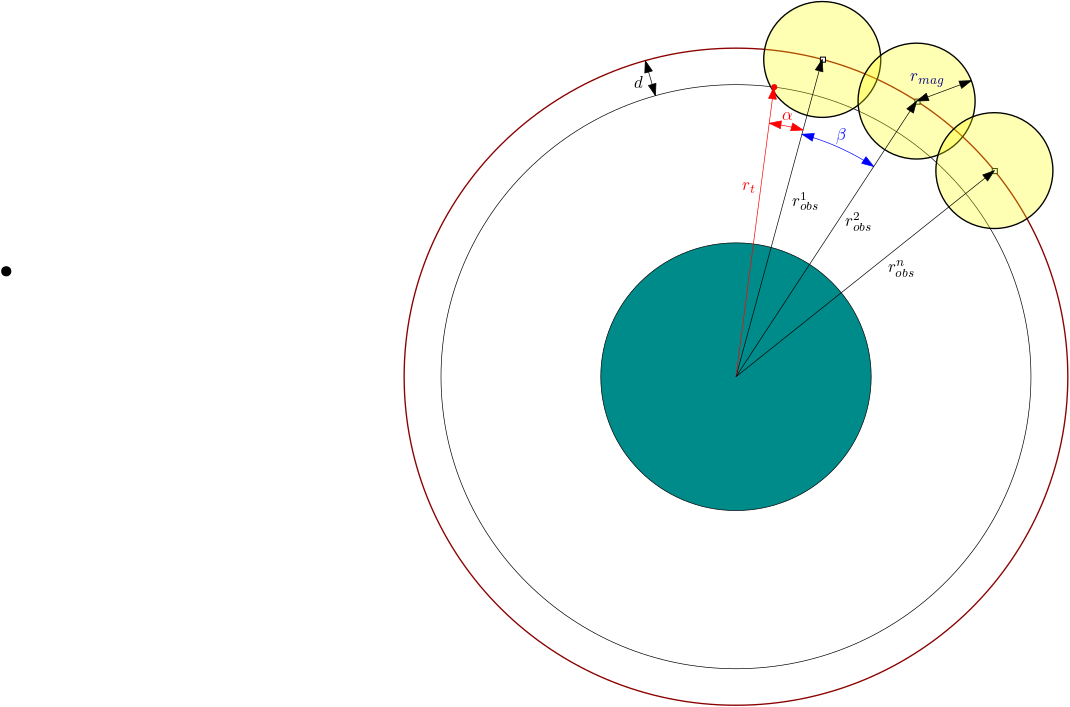
\includegraphics[width=0.6\columnwidth]{Figures/orbitas.png}
\caption{Observers and target orbits configuration}
\label{fig: orbitas-coplanarias}
\end{figure}
The first of these functions, namely \textit{generate\_position\_1st\_obs.m}, takes the lead in constructing the first observer initial position within the specified orbit, drawing parameters from the configuration file. The observer is placed at an angular distance denoted as $\alpha$ from the target.

Afterwards, a complementary function, \textit{generate\_position\_N\_obs.m}, was conceptualized to handle the placement of the remaining observers within the same orbit. This function defines an angular separation denoted as $\beta$ between the observers. It is worth emphasizing that both $\alpha$ and $\beta$ distances are inherently linked to the observer's effective sensor range, defined in the simulation as the radius of the visibility sphere.

It is crucial to highlight that the developed functions are designed to provide both Above the Horizon (ATH) and Below the Horizon (BTH) coverage, as elucidated in \cite{ATH-BTH}. The distinction in positioning arises from the observer's orbital semi-major axis concerning that of the target. When the observer is in an orbit with a semi-major axis greater than that of the target, it will exhibit a lower orbital velocity. To extend the observation time, the observers are strategically positioned with a true anomaly ($\nu$) greater than that of the target, given by $\nu_{obs_1} = \nu_t + \alpha$. Conversely, when the observer is in a lower orbit (providing ATH coverage), it will have a higher orbital velocity. To maximize the observation window in this scenario, the observers are situated with a true anomaly given by $\nu_{obs_1} = \nu_t - \alpha$. This strategic placement ensures comprehensive coverage by adapting to the inherent differences in orbital dynamics.

The nuanced approach to observer positioning becomes evident in the following code snippet:

\begin{lstlisting}[language=Matlab, caption= Excerpt of function \textit{generate\_position\_1st\_obs.m}.]
    function [r, v] = generate_1st_obs_pos(rt, vt, d)
    % Initialize output arrays
    r = zeros(3, 1);
    v = zeros(3, 1);

    % Extract Keplerian elements from the target state vectors
    [a_t, ecc_t, inc_t, RAAN_t, argp_t, nu_t] = ijk2keplerian(rt, vt);

    % Constants, define as wanted
    radius_coverage_sph = 1000000; % [m]this is a function of the magnitude
    initial_offset_o1_t = 10000;

    % Compute adjusted semi-major axis for observers
    a_obs = a_t + d;

    % Compute initial angular offset between the target and the first
    % observer
    alpha = acosd((a_obs^2 + a_t^2 - initial_offset_o1_t^2) / (2 * a_obs * a_t));
    if ~isreal(alpha)
        alpha = 0;
    else
        alpha = mod(alpha, 360);
    end
    % Determine true anomaly for observer 1, with the offset stated
    % previously
    if a_obs > a_t
        nu_obs1 = mod(nu_t + alpha, 360);
    else
        nu_obs1 = mod(nu_t - alpha, 360);
    end

    % Convert observer 1's Keplerian elements to Cartesian coordinates
    [r, v] = keplerian2ijk(a_obs, ecc_t, inc_t, RAAN_t, argp_t, nu_obs1);
end
\end{lstlisting}

The simulation workflow continues by propagating the initial positions of both the observers and the target along their respective orbits, leveraging the Keplerian orbit equation,
\begin{equation}
    \label{eq:state}
    \left\{\begin{aligned}\dot{x}\\\dot{y}\\\dot{z}\\\ddot{x}\\\ddot{y}\\\ddot{z}\end{aligned}\right\}=\left\{\begin{aligned}\dot{\boldsymbol{r}}&\\-\frac{\mu}{r^3}\boldsymbol{r}&+a_p\end{aligned}\right\}.
\end{equation}


In this particular case, the consideration of acceleration attributable to perturbations, denoted as $a_p$, has not been directly incorporated into the analysis. Rather, the introduced noise has been conceptualized as a surrogate for perturbations in the system.

The numerical Runge-Kutta 4 scheme is employed to ensure accurate and stable propagation, as given by the following equations:
\begin{equation}
    \begin{aligned}
        &X_{n+1} =X_n+\frac {\Delta t}{6}\left(k_1+2k_2+2k_3+k_4\right),  \\
        &t_{n+1} =t_n+\Delta t , \quad, with n=0, 1, 2, 3...,\\
    \end{aligned}
\end{equation}
where $X = (x, y, z,\dot{x}, \dot{y},\dot{z})$ represents the state vector, which comprises the position $r=(x, y, z)^T$ and the velocity $v=(\dot{x}, \dot{y},\dot{z})$ , $t$ denotes time, and $k_1, k_2, k_3,$ and $k_4$ are intermediary values calculated as per the Runge-Kutta method,\\
\begin{equation}
    \begin{aligned}
        &k_{1} =f(t_{n},X_{n}),  \\
        &k_{2} =f\biggl(t_{n}+\frac{\Delta t}{2},X_{n}+\Delta t\frac{k_{1}}{2}\biggr),  \\
        &k_{3} =f\biggl(t_{n}+\frac{\Delta t}{2},X_{n}+\Delta t\frac{k_{2}}{2}\biggr),  \\
        &k _4=f(t_{n}+\Delta t,y_{n}+\Delta tk_{3}). \\
        \end{aligned}
\end{equation}
After propagating the orbits, a controlled positioning error, alongside attitude and directional errors, is introduced to the observer. This step is crucial for simulating potential deviations in the measurements that may arise from real-world scenarios. The introduced errors follow a bounded distribution, ensuring a realistic yet manageable level of uncertainty.
Both the perturbed and unperturbed datasets are stored as outputs of the simulator. 

\subsubsection{Estimator Algorithm: Unscented Kalman Filter}


As highlighted in the introduction, a fundamental achievement of Space Situational Awareness (SSA) systems revolves around the determination of Resident Space Object (RSO) size and position. This estimation, often articulated through Keplerian parameters, Cartesian coordinates, or alternative representations, plays a pivotal role in predicting the RSO's future position with a desirable degree of precision. In this study, a streamlined adaptation of the algorithm presented in \cite{linares} has been employed to focus on estimating the variables inherent in the state vector $X$.

The process of estimating state variables within the state vector is a nuanced task, and it is typically approached using well-established algorithms. Among these, two extensions of the Standard Kalman Filter (KF), namely the Extended Kalman Filter (EKF) \cite{EKF} and the Unscented Kalman Filter (UKF) \cite{UKF} stand out as widely adopted methodologies. Both of these algorithms inherently consist of two principal steps:

\begin{itemize}
    \item \textbf{The prediction step}: in the initial phase, the algorithm uses the system's propagation model (in this case RK4) to forecast its future state (referred to as the a priori state). During this step, the associated covariance matrix for the state variables is also projected forward.
    \item \textbf{Correction step}: In this subsequent phase, the algorithm compares the real system's measurement with the predicted one based on the earlier forecasted state. Using the outcome of this comparison and the optimal correction gain, the predicted state is adjusted (referred to as the a posteriori state), and concurrently, the covariance matrix is updated.
\end{itemize}

Presently, due to considerations outlined in \cite{ref:UKFvsEKF}, the decision has been made to employ the Unscented Kalman Filter (UKF)whose formulation will be briefly summarized shortly. Nevertheless, owing to the enhanced modular structure of the code, the substitution of the estimator would be a seamless process, contingent upon the introduction of an alternative estimation function into the designated folder.

\paragraph{Formulación del UKF}

Consider the following non-linear system:
\begin{equation}\begin{aligned}\boldsymbol{x}_{k+1}&=f(\boldsymbol{x}_k,\boldsymbol{v}_k)\\\boldsymbol{y}_{k+1}&=h(\boldsymbol{x}_{k+1},u_k)\end{aligned}\end{equation}
 
Here, $f(\boldsymbol{x})$ represents the function delineating the evolution of the state variables, where in the present context, it corresponds to \autoref{eq:state}. The symbols $\boldsymbol{y}$ denote system measurements, $h$ denotes the measurement function, and $v, u$ signify process and measurement errors, respectively. Furthermore, $k$ is an arbitrary time instant.

Assuming a known (or accurately estimated) covariance matrix of the state variables ($\boldsymbol{P}_k$) at the given time, the calculation of sigma points is as follows:
\begin{equation}\begin{aligned}
    &\chi_{k}^{0} =x_{k}  \\
    &\chi_{k}^{i} =\boldsymbol{x}_k+\left(\sqrt{(n+\lambda)\mathbf{P}_k}\right)_i\quad i=1...n  \\
    &\chi_{k}^{i} =x_{k}+\left(\sqrt{(n+\lambda)\mathbf{P}_{k}}\right)_{i-n}\quad i=n+1\ldots2n, 
\end{aligned}\end{equation}
Here, $\chi$ denotes the sigma points, $n$ stands for the dimension of the state vector, and $\lambda$ represents a scale parameter calculated as:
\begin{equation}
\lambda = \alpha^2(n+\kappa)-n,
\end{equation}
Parameters $\alpha$ and $\kappa$ necessitate adjustment based on the filter's requirements. Subsequently, the calculation of weights associated with the sigma points ($W$) unfolds as follows:
\begin{equation}\begin{aligned}W^{0,m}&=\frac\lambda{\lambda+n}\\W^{0,c}&=\frac\lambda{\lambda+n}+1-\alpha^2+\beta\\W^{i,m}&=W^{i,c}=\frac\lambda{2(\lambda+n)}\quad i=1...2n\end{aligned},\end{equation}
where $\beta$ emerges as another parameter of the estimator.


After determining the sigma points and their corresponding weights, the next step involves computing the predicted state and covariance matrix:
\begin{equation}\begin{aligned}\mathbf{x}_{k+1}^-&=\sum_{i=0}^{2n}W_i^mf(\chi_k^i)\\\mathbf{P}_{k+1}^-&=\sum_{i=0}^{2n}W_i^c\left(\chi_{k+1}^{-,i}-\mathbf{x}_{k+1}^-\right)\left(\chi_{k+1}^{-,i}-\mathbf{x}_{k+1}^-\right)^T+\mathbf{Q}\end{aligned}\end{equation}
where $\boldsymbol{Q}$ is a matrix that models the system noise. This first prediction step keeps estimating the estate variables until there is a new experimental (or simulation) measurement available, starting the correction step. When this happens, the expected state is calculated as follows:

\begin{equation}\begin{aligned}Y_{k+1}^{-,i}&=h(\chi_{k+1}^{-,i})\\y_{k+1}^-&=\sum_{i=0}^{2n}W_i^mh(\chi_{k+1}^{-,i}).\end{aligned}\end{equation}

Note that $\boldsymbol{Y}$ is the computation of the expected measurement's sigma points. Having the expected measurement, the corrected state can be calculated as:

\begin{equation}\begin{gathered}
    \text{P} _{\boldsymbol{y}\mathbf{y}}=\sum_{i=0}^{2n}W_{i}^{c}\left(Y_{k+1}^{-,i}-\boldsymbol{y}_{k+1}^{-}\right)\Bigl(Y_{k+1}^{-,i}-\boldsymbol{y}_{k+1}^{-}\Bigr)^{\mathrm{T}}+\mathbf{R} \\
    \mathbf{P}_{xy}=\sum_{i=0}^{2n}W_{i}^{c}\left(\chi_{k}^{i}-\boldsymbol{x}_{k+1}^{-}\right)\left(Y_{k+1}^{-,i}-\boldsymbol{y}_{k+1}^{-}\right)^{\mathrm{T}} \\
    K=\mathbf{P}_{xy}\mathbf{P}_{yy}^{-1} \\
    x_{k+1}=x_{k+1}^{-}+K(y_{k+1}-y_{k+1}^{-}) \\
    \mathbf{P}_{k+1}=\mathbf{P}_{k+1}^{-}-K\mathbf{P}_{yy}K^{\mathrm{T}} .
\end{gathered}\end{equation}
Here, $\boldsymbol{R}$ is a matrix refresenting the noise of the measurement and $K$ is the filter gain to update the sytem and covariance matrix

To use the filter in the most versatile manner possible, it is advantageous that the acquired measurements are independent of the sensors capturing them. Otherwise, it would be neccessary to model the errors introduced by each individual sensor, adding a layer of complexity to the estimation process. Consequently, a decision is made to preprocess the actual measurements, obtained in this case from the simulation, transforming them from the pixel values of light that the sensors would capture to more meaningful quantities for the problem at hand. These transformed measurements specifically entail the unit vector pointing towards the Resident Space Object (RSO), denoted as $\hat{\rho}$, and the apparent magnitude $m$. By adopting this preprocessing step, not only is the relevance of the measurements enhanced with respect to the problem domain, but it also circumvents the introduction of noise from diverse sensor equipment, ensuring a more robust and accurate estimation process. The process mede to obtain these values is further explained in \autoref{sec:fotometria}









% \section*{Unscented Kalman Filter Algorithm for Space-Based Space Situational Awareness}



% \section{VENTAJAS MODULAR CODING}
% In the field of space-based Space Situational Awareness (SSA), the structural design of software code is paramount to ensuring efficiency, maintainability, and extensibility. The adoption of a modular coding paradigm proves particularly instrumental in providing a systematic and organized framework for software development. This paper underscores the significance of modular coding, specifically focusing on its application in decomposing complex SSA systems into manageable and interdependent modules, each encapsulating distinct functionalities.

% One fundamental advantage of modular coding in SSA resides in its facilitation of code maintenance and scalability. By segregating different aspects of the codebase into modular units, such as the separation of scientific algorithms from simulation components, the overall system becomes more comprehensible and easier to manage. This clear separation allows for targeted modifications or enhancements in response to evolving requirements without necessitating extensive changes to the entire codebase. Consequently, maintenance efforts are streamlined, reducing the likelihood of unintended side effects and minimizing the risk of introducing errors during updates.

% Moreover, the separation of the scientific and simulation components within the code structure contributes to enhanced code reusability. Isolating scientific algorithms into dedicated modules fosters a more versatile and adaptable codebase. This modularity enables the reuse of well-defined scientific functionalities across diverse simulations or applications, promoting efficiency in development and contributing to a more sustainable and flexible software architecture.

% In the formal and scientific context, the strategic separation of the science and simulation aspects adheres to best practices in software engineering, offering both methodological and practical advantages. This approach not only supports the comprehensibility and maintainability of the codebase but also reinforces the adaptability and extensibility of the software framework, essential attributes in the dynamic and evolving field of space-based SSA.

